\section{Weitere Irradiance Map Ergebnisse} % (fold)
\label{sec:weitere_irradiance_map_ergebnisse}

	\begin{figure}[H]
		\begin{subfigure}[b]{0.5\textwidth}
			\center
			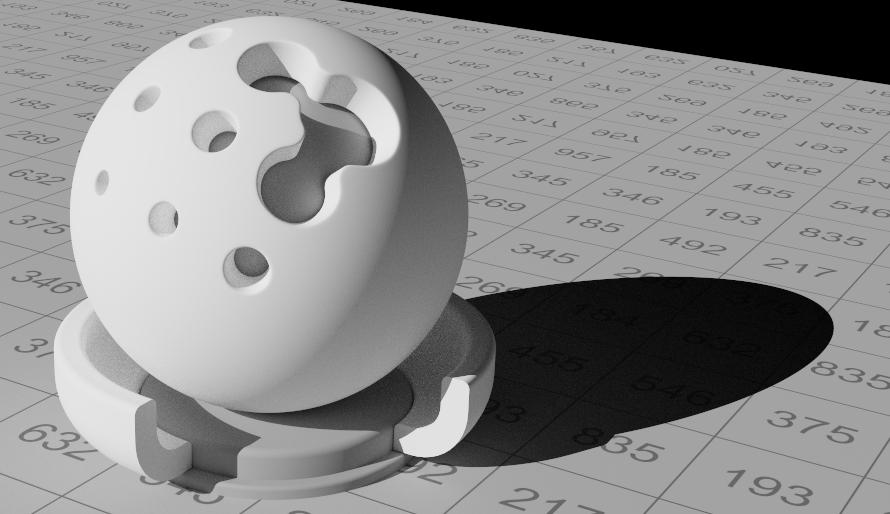
\includegraphics[width=0.95\textwidth]{pic/irrmap-shaderball-ref.png}
			\caption{Path Tracing}
			\label{subfig:irrmap-shaderball-ref}
		\end{subfigure}
		\begin{subfigure}[b]{0.5\textwidth}
			\center
			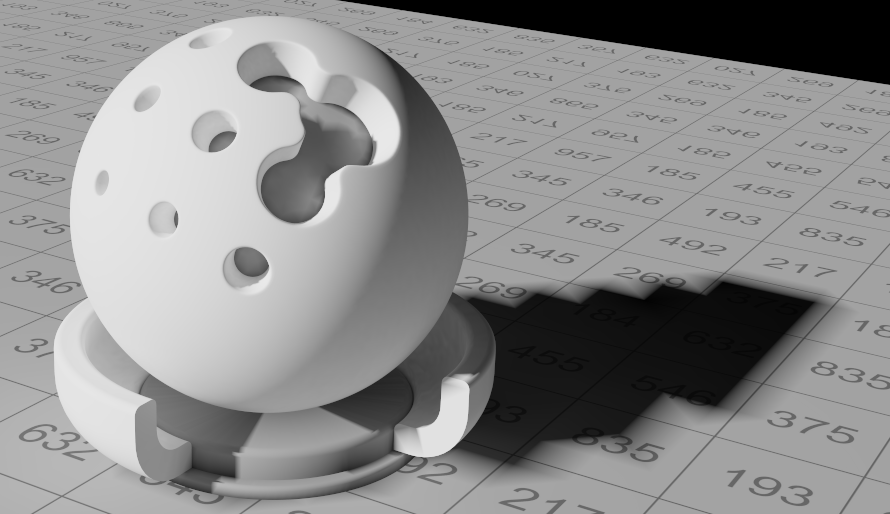
\includegraphics[width=0.95\textwidth]{pic/irrmap-shaderball-vmap.png}
			\caption{Vertex Lighting}
			\label{subfig:irrmap-shaderball-vmap}
		\end{subfigure}
		\medskip \\
		\begin{subfigure}[b]{0.5\textwidth}
			\center
			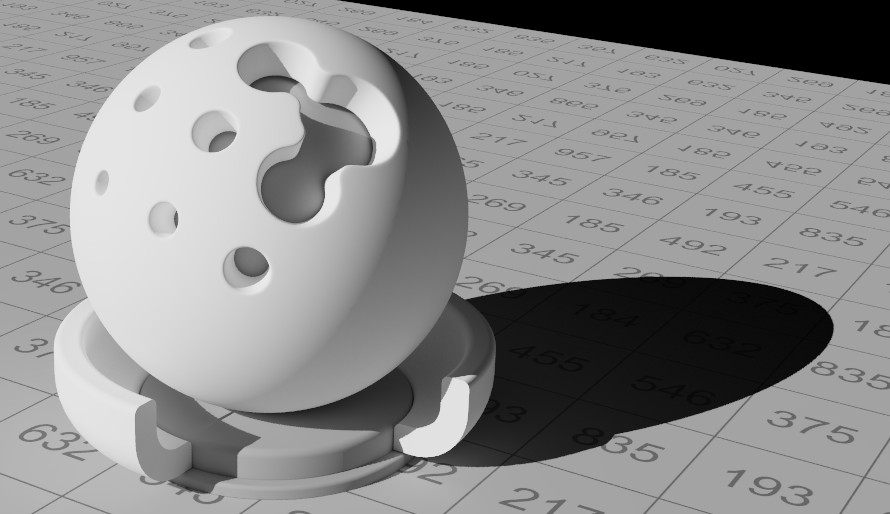
\includegraphics[width=0.95\textwidth]{pic/irrmap-shaderball-irrmap.png}
			\caption{Irradiance Map}
			\label{subfig:irrmap-shaderball-irrmap}
		\end{subfigure}
		\begin{subfigure}[b]{0.5\textwidth}
			\center
			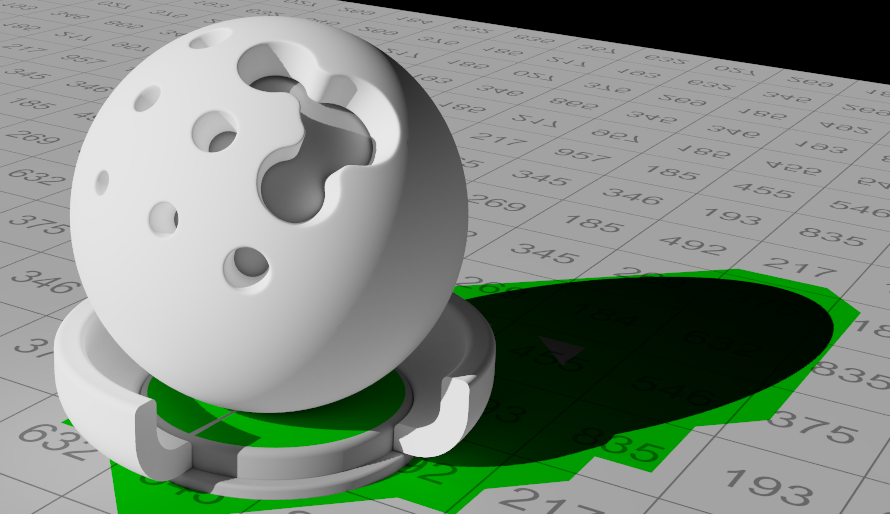
\includegraphics[width=0.95\textwidth]{pic/irrmap-shaderball-irrmap-order.png}
			\caption{Irradiance Map Ordnung}
			\label{subfig:irrmap-shaderball-irrmap-order}
		\end{subfigure}
		\caption[Irradiance-Map der \enquote{Shaderball}-Szene mit direktionaler Lichtquelle]{Die Bilder zeigen die \enquote{Shaderball}-Szene mit einer direktionalen Lichtquelle unter Verwendung von Path Tracing als Referenzbild, von Vertex Lighting und der Irradiance Map. Für die adaptive Irradianzschätzung wurden eine obere Fehlerschranke von $1\unit{\%}$ und maximal $2^{14}$ Samples verwendet. Die Irradiance Map wurde durch circa $15.6\cdot10^6$ Messpunkte bestimmt, die insgesamt $59.7\unit{MiB}$ einnehmen. Die obere Fehlerschranke betrug $2.5\unit{\%}$ und die maximale Ordnung $2^7$. Die Generierung benötigte $11500\unit{s}$. Die grün markierten Bereich in \ref{subfig:irrmap-shaderball-irrmap-order} stellen Dreiecke mit einer Ordnung größer $63$ dar.}
		\label{fig:irrmap-shaderball}
	\end{figure}

	\begin{figure}[H]
		\begin{subfigure}[b]{0.5\textwidth}
			\center
			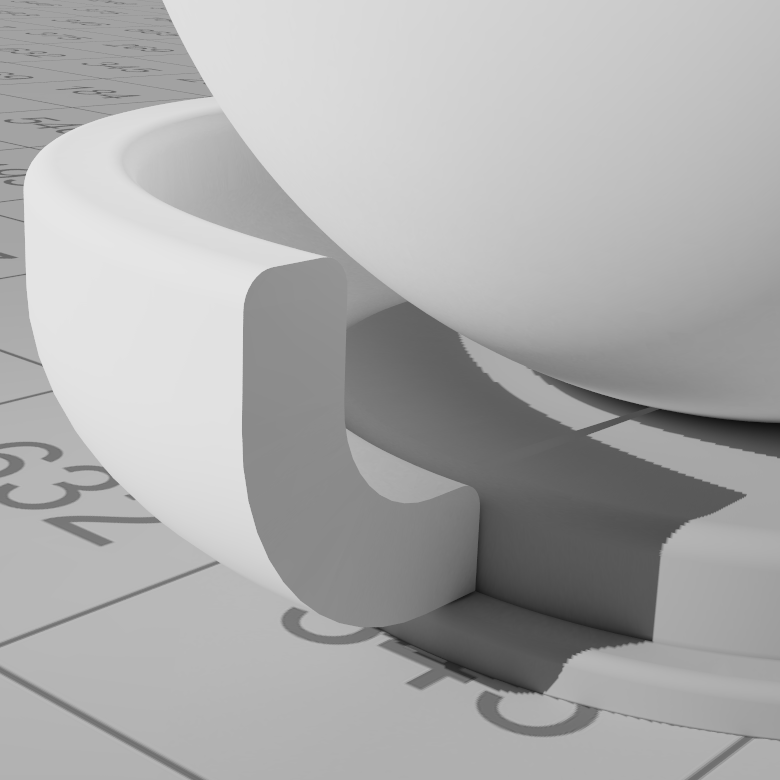
\includegraphics[width=0.95\textwidth]{pic/irrmap-shaderball2-irrmap.png}
			\caption{Irradiance Map}
		\end{subfigure}
		\begin{subfigure}[b]{0.5\textwidth}
			\center
			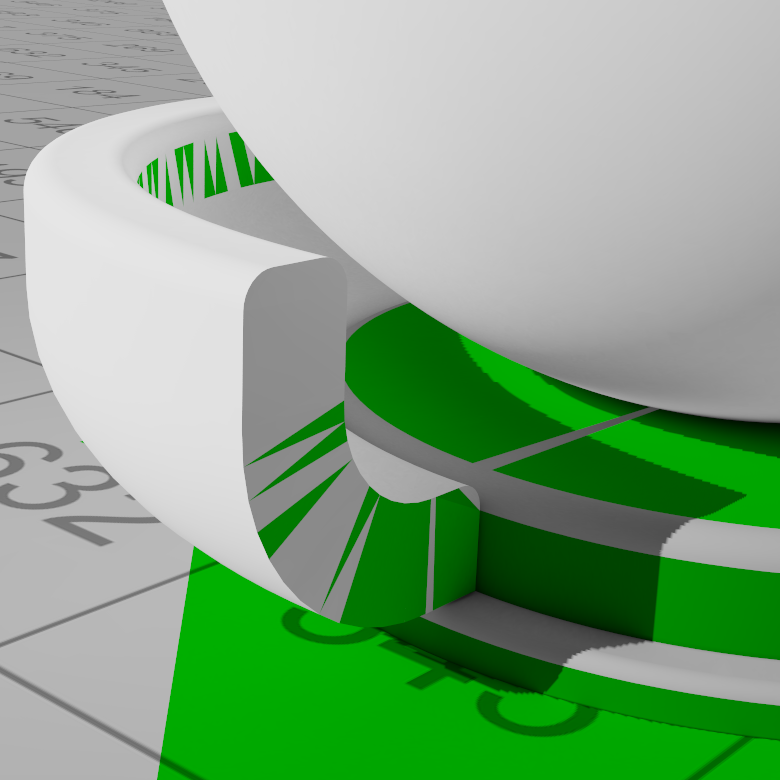
\includegraphics[width=0.95\textwidth]{pic/irrmap-shaderball2-irrmap-order.png}
			\caption{Irradiance Map Ordnung}
			\label{subfig:irrmap-shaderball2-irrmap-order}
		\end{subfigure}
		\caption[Irradiance Map Fehler der \enquote{Shaderball}-Szene mit direktionaler Lichtquelle]{Die Bilder zeigen die \enquote{Shaderball}-Szene aus Abbildung \ref{fig:irrmap-shaderball} aus einem anderen Blickwinkel. Die grün markierten Bereiche in \ref{subfig:irrmap-shaderball2-irrmap-order} stellen Dreiecke mit einer Ordnung größer $8$ dar. Es ist erkennbar, dass am Rand des harten Schattens Aliasing-Artefakte entstehen. Weiterhin gibt es ein Dreieck auf der unteren Platte, welches einen fehlerhaften Schattenverlauf zeigt. Hier bewertete das verwendete Fehlermaß das Dreieck falsch, da die Irradianz eine hohe Variation besitzt.}
		\label{fig:irrmap-shaderball2}
	\end{figure}

% section weitere_irradiance_map_ergebnisse (end)